\section{系统调用机制与中断}

中断是一种异步事件,它可以打断正在执行的程序并转移到处理中断的程序(中断处理程序)。
中断可以来自外部设备(如硬件中断)或软件(如系统调用)。中断机制是操作系统用来响应和处理中断的一种机制,
其中涉及中断向量表、中断控制器、中断处理程序等概念。

系统调用是中断的一种,通常情况下,U态的中断包括了系统调用,系统调用陷入内核态后,
将会调用SBI call来执行具体的内容。下面的\autoref{fig:syscall和SBI区别}清晰地展示了这两种中断的区别及联系。

\begin{figure}[htb]
    \centering
    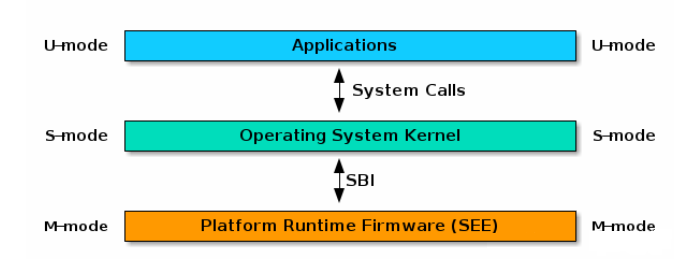
\includegraphics[width=\textwidth]{figures/03-03-syscall和SBI区别.png}
    \caption{
        syscall和SBI区别
    }
    \label{fig:syscall和SBI区别}
\end{figure}

系统调用是应用程序向操作系统请求服务的一种机制。应用程序无法直接访问操作系统内核的代码和数据结构,
因此需要通过系统调用来请求操作系统的服务。例如,在Linux操作系统中,应用程序可以通过系统调用请求创建新的进程、
读写文件、网络通信等操作。

同时,RISC-V使用SBI(Supervisor Binary Interface)作为系统调用的接口,提供了一组标准的系统调用函数,
包括控制台输出、内存分配、时钟等服务。

从系统调用以及中断的角度考虑,RISC-V使用TVEC(Trap Vector Base Address)寄存器来指定中断向量表的基地址,
中断向量表存储了中断处理程序的入口地址。当发生中断时,CPU会自动跳转到相应的中断处理程序,
并在处理完成后返回到中断前的指令位置。RISC-V还提供了一些相关的指令和寄存器,用于中断的使能、屏蔽和处理。

\autoref{fig:RISC-V的系统调用处理流程图}是riscv架构下对系统调用的处理流程。

\begin{figure}[htb]
    \centering
    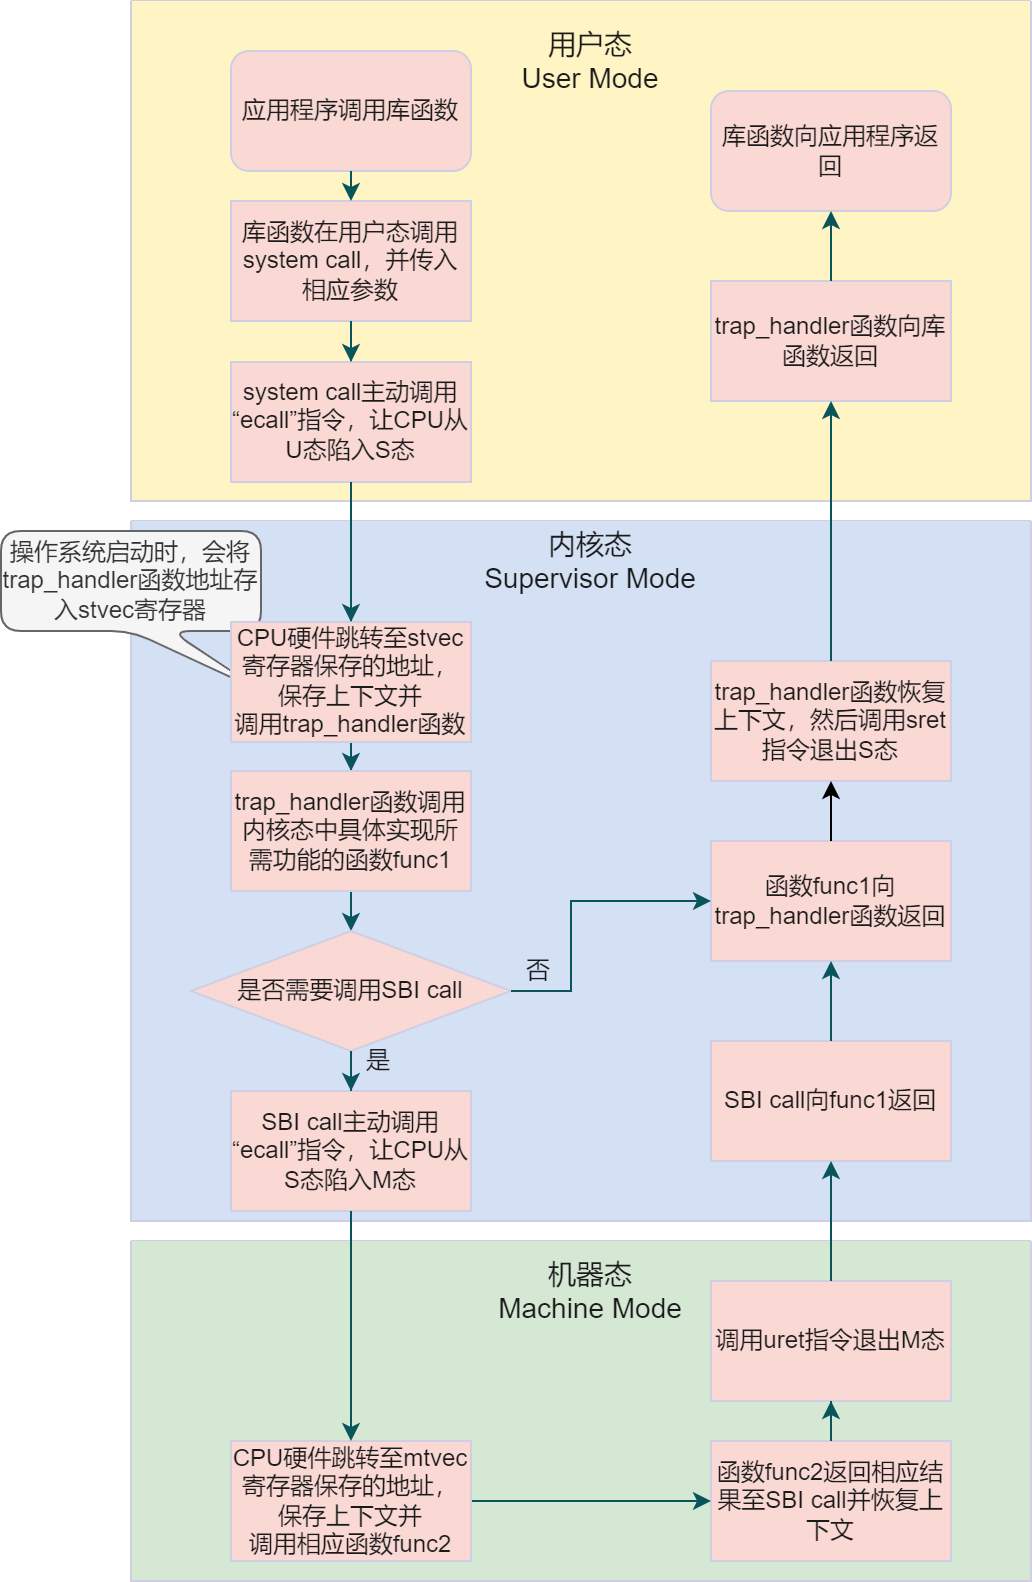
\includegraphics[width=0.5\textwidth]{figures/03-03-RISC-V的系统调用处理流程图.png}
    \caption{
        RISC-V的系统调用处理流程图
    }
    \label{fig:RISC-V的系统调用处理流程图}
\end{figure}

从本节开始,我们将正式开始学习NPUcore对于系统调用的真正处理和实现。
为了确保知识的合理递进,我们将其中最重要的内容分为了下面几个小节:

\begin{itemize}
    \item Trap及中断使能
    \item 系统调用与ecall指令
    \item 设置stvec寄存器及编写trap_handle函数
    \item 利用汇编实现上下文保存与恢复
    \item RustSBI简介及调用RustSBI
\end{itemize}

\subsection{Trap及中断使能}

\subsubsection{Trap的概念及其作用}

在上文中我们提到,系统调用是trap的一种,因此我们要了解系统调用,必须先了解trap是什么。

trap的3种类型:
\begin{enumerate}
    \item 主动的陷入:system call
    \item 外设中断处理:鼠标、键盘响应
    \item 运行时的意外:error、溢出、除0等
\end{enumerate}

每个RISC-V CPU都有一组控制寄存器,内核通过向这些寄存器写入内容来告诉CPU如何处理陷阱,
内核可以读取这些寄存器来明确已经发生的陷阱。RISC-V文档包含了完整的内容。riscv.h(kernel/riscv.h:1)
包含在NPUcore中使用到的内容的定义。\autoref{table:重要寄存器概述}是最重要的一些寄存器概述:

\begin{table}[h]
    \centering
    \caption{重要寄存器概述}
    \label{table:重要寄存器概述}
    \begin{tabularx}{0.8\textwidth}{|p{2cm}|X|}
    \hline
    \textbf{寄存器名称} & \textbf{功能}                                                     \\\hline
    stvec    & 内核在这里写入其陷阱处理程序的地址,RISC-V跳转到这里处理陷阱                     \\\hline
    sepc     & 当发生陷阱时,RISC-V会在这里保存程序计数器pc(因为pc会被stvec覆盖)              \\\hline
    sret     & (从陷阱返回)指令会将sepc复制到pc,内核可以写入sepc来控制sret的去向              \\\hline
    scause   & RISC-V在这里放置一个描述陷阱原因的数字                                         \\\hline
    sscratch & 内核在这里放置了一个值,这个值在陷阱处理程序一开始就会派上用场                    \\\hline
    sstatus  & 其中的SIE位控制设备中断是否启用。如果内核清空SIE,RISC-V将推迟设备中断,          
               直到内核重新设置SIE。SPP位指示陷阱是来自用户模式还是管理模式,并控制sret返回的模式 \\\hline
    \end{tabularx}
\end{table}

\subsubsection{使能中断}

使能中断指的是在CPU中打开中断处理的能力。如果中断被禁用,即使有中断请求发生,CPU也不会执行中断处理程序,
而是继续执行当前的任务,直到中断被启用为止。一旦中断被启用,当有中断请求发生时,
CPU会在适当的时候挂起当前的任务,跳转到中断处理程序,执行完毕后再返回到原来的任务。

在RISC-V架构中,使能中断可以通过设置sstatus寄存器下的SIE位来打开或关闭的中断使能。
当相应的寄存器被置为1时,对应的中断将被使能。

\begin{figure}[htb]
    \centering
    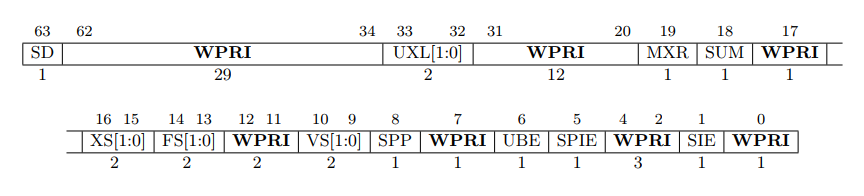
\includegraphics[width=\textwidth]{figures/03-03-SXLEN=64时S-mode下的状态寄存器(sstatus).png}
    \caption{
        SXLEN=64时S-mode下的状态寄存器(sstatus)
    }
    \label{fig:SXLEN=64时S-mode下的状态寄存器(sstatus)}
\end{figure}

在NPUcore中,为了确保中断与系统调用可用,我们利用RustSBI进行了如下的操作:

\begin{lstlisting}[language={Rust}]
unsafe {
    riscv::register::sstatus::set_sie();
}
\end{lstlisting}

该操作实际上是对sstatus寄存器的低1位赋值为1,这样便打开了中断使能。

\subsection{系统调用与ecall指令}

在RISC-V架构下,系统调用是通过ecall指令来触发的。ecall指令是一条特殊的指令,当我们在U态执行ecall指令时,
会跳转到STVEC寄存器中函数地址指定的中断处理程序,即系统调用处理程序
(若是在S态触发ecall,则会跳转到mtvec存储的函数地址),进行相应的操作。
ecall指令一般用来触发一些特殊的操作,比如系统调用、中断、异常等。

当我们在U态利用系统调用出发ecall指令后,需要进行相应的操作,比如将参数传递到内核态,由内核态进行相应的操作,
然后再将结果返回给用户态。在系统调用发生时,需要将当前用户态的上下文保存起来,这样在系统调用完成后,
CPU就可以从保存的上下文中恢复用户态的执行状态。

接下来,我们通过NPUcore具体的代码实例来学习如何利用ecall指令来完成系统调用。

我们以write系统调用为例,来详细描述系统调用的具体流程。

\subsubsection{用户态进程调用syscall}

\begin{itemize}
    \item 应用程序调用位于user/src/usr_call.rs中被包装好的write函数;
    \item write函数调用位于user/src/usr_call.rs中的sys_write函数;
\end{itemize}

应用程序如何想使用操作系统为其提供的服务,最直接的办法就是调用操作系统提供的库函数。

NPUcore的设计正是如此,我们将syswrite函数进行了一次包装,放在user/src/usr_call.rs中,模拟库函数,
见\autoref{code:usr call write}。

我们对sys_write传递两个参数,分别是文件描述符fd以及缓冲区指针buf。

\begin{lstlisting}[language={Rust}, label={code:usr call write},
    caption={usr_call.rs:write}]
pub fn write(fd: usize, buf: &[u8]) -> isize {
    sys_write(fd, buf)
}
\end{lstlisting}

\begin{itemize}
    \item sys_write函数调用位于user/src/usr_call.rs中的syscall函数;
\end{itemize}

见\autoref{code:usr call sys write},我们的包装类似于lib库函数,利用sys_write函数来调用syscall。

\begin{lstlisting}[language={Rust}, label={code:usr call sys write},
    caption={usr_call.rs:sys_write}]
pub fn sys_write(fd: usize, buffer: &[u8]) -> isize {
    syscall(SYSCALL_WRITE, [fd, buffer.as_ptr() as usize, buffer.len()])
}
\end{lstlisting}

\subsubsection{syscall调用ecall指令陷入内核态}

syscall函数中内联的汇编函数执行了ecall,陷入内核态。每一个syscall都有4个参数,
第一个参数代表着系统调用的id,NPUcore的系统调用标识完全遵循linux标准,因此可以方便地兼容linux操作系统的应用程序。
其余三个参数供每个系统调用进行灵活选择。

\begin{lstlisting}[language={Rust}, label={code:syscall},
    caption={syscall}]
fn syscall(id: usize, args: [usize; 3]) -> isize {
    let mut ret: isize;
    unsafe {
        asm!(
            "ecall",
            inlateout("x10") args[0] => ret,
            in("x11") args[1],//分别把参数放进a1、a2、a7
            in("x12") args[2],
            in("x17") id
        );
    }
    ret
}
\end{lstlisting}

见\autoref{code:syscall},在第五行,第一条指令就是ecall指令,我们在此调用ecall指令触发trap,使得程序陷入内核态
第六行的inlateout指令有两个作用:一是把args[0]放进a0寄存器;二是在程序返回后x10寄存器会作为返回值。
接下来三行就是参数的传递。

至此,我们已经完成了系统调用在用户空间中应该进行的操作。

\subsection{设置stvec寄存器与编写trap_handle函数}

在用户态进程调用ecall进入内核态后,CPU将会自动进行如下操作:

\begin{itemize}
    \item sstatus 的 SPP 字段会被修改为 CPU 当前的特权级(U/S)。
    \item sepc 会被修改为 Trap 处理完成后默认会执行的下一条指令的地址。
    \item scause/stval 分别会被修改成这次 Trap 的原因以及相关的附加信息。
    \item CPU 会跳转到 stvec 所设置的 Trap 处理入口地址,并将当前特权级设置为 S ,然后从Trap 处理入口地址处开始执行。
\end{itemize}

在这些操作中,我们最需要关心的是第四点。

尽管上文已经提到了stvec寄存器的具体功能,但仍然在这强调一下该寄存器的具体作用:
在RISC-V架构中,中断控制器寄存器写入的是中断向量表的基地址(Base Address)。
stvec寄存器用于存储中断向量表的基地址,并指定了中断向量表的模式(Direct Mode或Vectored Mode)。
当中断处理器接收到一个中断信号时,会根据stvec寄存器的值,自动跳转到中断向量表中对应的中断处理程序的入口地址。

因为硬件实现了自动跳转到stvec寄存器的功能,因此接下来我们只需要考虑如何往stvec寄存器中写入内容,以及写入什么内容。
这两个问题的回答正是我们这一小节的主题——设置stvec寄存器及编写trap_handle函数。

\subsubsection{设置stvec寄存器}

我们应该向stvec写入什么呢?答案是显而易见的——中断处理函数。

其实,在操作系统初始化的时候,就已经修改了 stvec 寄存器来指向正确的 Trap 处理入口点,
见\autoref{code:set user trap entry}。

\begin{lstlisting}[language={Rust}, label={code:set user trap entry},
    caption={set_user_trap_entry}]
fn set_user_trap_entry() {
    unsafe {
        stvec::write(TRAMPOLINE as usize, TrapMode::Direct);
    }
}
\end{lstlisting}

这里引入了一个外部符号 TRAMPOLINE(意为跳板) ,并将 stvec 设置为 Direct 模式指向它的地址。
在 os/src/trap/trap.S 中实现 Trap 上下文保存/恢复的汇编代码,分别用外部符号 __alltraps 和 __restore 标记为函数,
并通过 global_asm! 宏将 trap.S 这段汇编代码插入进来。

为什么我们不直接将__alltraps符号写入stvec寄存器,而是要建立一个跳板?
使用跳板是为了解决这样一个问题:
在开启分页模式之后__alltraps的实际程序入口并不是一个特定值,而是取决于所处平台的不同(qemu/k210/u740)
以及在编译器/汇编器/链接器进行后端代码生成和链接形成最终机器码时设置好的此指令的地址。

从上文中我们可以知道,在编写 trap.S 中的整段汇编代码时,我们将这段代码放置在 .text.trampoline 段。

该符号在os/src/linker-k210.ld、os/src/linker-fu740.ld及os/src/qemu.ld被连接,
并在调整内存布局的时候将它对齐到代码段的一个页面中,见\autoref{code:linker-xxx-.ld}。

\begin{lstlisting}[label={code:linker-xxx-.ld},
    caption={linker-xxx-.ld}]
stext = .;
.text : {
    *(.text.entry)
    . = ALIGN(4K);
    strampoline = .;
    *(.text.trampoline);
    . = ALIGN(4K);
    ssignaltrampoline = .;
    KEEP(*(.text.signaltrampoline));
    . = ALIGN(4K);
    *(.text .text.*)
}
\end{lstlisting}

这样,这段汇编代码放在一个物理页帧中,且 __alltraps 恰好位于这个物理页帧的开头,
其物理地址被外部符号 strampoline 标记。在开启分页模式之后,内核和应用代码都只能看到各自的虚拟地址空间,
而在它们的视角中,这段汇编代码都被放在它们各自地址空间的最高虚拟页面上,
由于这段汇编代码在执行的时候涉及到地址空间切换,故而被称为跳板页面。

这样就可以解释为何在 __alltraps 中需要借助寄存器 jr 而不能直接 call trap_handler 了。
因为在内存布局中,这条 .text.trampoline 段中的跳转指令和 trap_handler 都在代码段之内,
汇编器(Assembler)和链接器(Linker)会根据 linker-qemu/k210.ld 的地址布局描述,设定跳转指令的地址,
并计算二者地址偏移量,让跳转指令的实际效果为当前 pc 自增这个偏移量。
但实际上由于我们设计的缘故,这条跳转指令在被执行的时候,它的虚拟地址被操作系统内核设置在地址空间中的最高页面之内,
所以加上这个偏移量并不能正确的得到 trap_handler 的入口地址。

在完成了这一步骤后,接下来将正式开始在S态中的中断处理流程。

\subsubsection{编写trap_handler函数}

在完成上文所述的设置stvec寄存器跳转地址后,我们将完成后续步骤:

\begin{itemize}
    \item 通过 __alltraps 将 Trap 上下文保存在内核栈上。
    \item 跳转到使用 Rust 编写的 trap_handler 函数完成 Trap 分发及处理。
    \item 当 trap_handler 返回之后,使用 __restore 从保存在内核栈上的 Trap 上下文恢复寄存器。
    \item 最后通过一条 sret 指令回到应用程序执行。
\end{itemize}

本节重点讲解其中的第二点,追踪NPUcore中trap_handler函数的具体实现流程并了解其核心思想。
由于该函数过长,这里只选取其中有关系统调用的部分进行讲解,见\autoref{code:trap handler}。

\begin{lstlisting}[language={Rust}, label={code:trap handler},
    caption={trap_handler}]
pub fn trap_handler() -> ! {
    set_kernel_trap_entry();
	//...
    let scause = scause::read();
    match scause.cause() {
        Trap::Exception(Exception::UserEnvCall) => {
            let mut cx = current_trap_cx();
            cx.gp.pc += 4;
            let result = syscall(
                cx.gp.a7,
                [cx.gp.a0, cx.gp.a1, cx.gp.a2, cx.gp.a3, cx.gp.a4, cx.gp.a5],
            );
            cx = current_trap_cx();
            cx.gp.a0 = result as usize;
        }
	//...
    trap_return();
}
\end{lstlisting}

在函数的开始,代码第2行,调用了set_kernel_trap_entry函数,在内核态的陷入是什么情况呢?
报错!这个函数定义了如果在内核态再发生Trap,会直接panic报错,是为了防止不正常的S->S态Trap的发生。

在第5行的match匹配,这个处理系统调用的子块函数做了三件事:
第一步,让pc+4,是为了跳转后能正确执行下一条指令。
第二步,把scause寄存器的值取出,调用os/src/syscall/mod.rs里面的syscall函数。
第三步,将返回值存入返回值寄存器a0中。

为什么在用户空间中有一个syscall函数,在内核空间中又会出现一个同名的syscall函数呢?
其实只有用户空间那个syscall才是我们平常意义上所说的系统调用,因为只有该syscall才调用了ecall指令,完成了trap操作。
而在内核空间中出现的syscall可以认为是对系统调用所需要完成的不同功能进行分发处理。

内核空间中出现的syscall在os/src/syscall/mod.rs中。
由于该函数过长,只选取其中少数几个的match项,见\autoref{code:syscall}。
示例该函数只是起一个根据系统调用号对操作进行分发的作用。

\begin{lstlisting}[language={Rust}, label={code:syscall},
    caption={syscall}]
pub fn syscall(syscall_id: usize, args: [usize; 6]) -> isize {
	//log
    let ret = match syscall_id {
        SYSCALL_GETCWD => sys_getcwd(args[0], args[1]),
        SYSCALL_DUP => sys_dup(args[0]),
        SYSCALL_DUP3 => sys_dup3(args[0], args[1], args[2] as u32),
        SYSCALL_FCNTL => sys_fcntl(args[0], args[1] as u32, args[2]),
        SYSCALL_IOCTL => sys_ioctl(args[0], args[1] as u32, args[2]),
       //...still more
    };
    ret
}
\end{lstlisting}

最后,在 trap_handler 完成 Trap 处理之后,调用 trap_return 返回用户态,见\autoref{code:trap return}。

\begin{lstlisting}[language={Rust}, label={code:trap return},
    caption={trap_return}]
fn set_user_trap_entry() {
    unsafe {
        stvec::write(TRAMPOLINE as usize, TrapMode::Direct);
    }
}

#[no_mangle]
pub fn trap_return() -> ! {
    set_user_trap_entry();
    let trap_cx_ptr = TRAP_CONTEXT;
    let user_satp = current_user_token();
    extern "C" {
        fn __alltraps();
        fn __restore();
    }
    let restore_va = __restore as usize - __alltraps as usize + TRAMPOLINE;
    unsafe {
        asm!(
            "fence.i",
            "jr {restore_va}",
            restore_va = in(reg) restore_va,
            in("a0") trap_cx_ptr,
            in("a1") user_satp,
            options(noreturn)
        );
    }
    panic!("Unreachable in back_to_user!");
}
\end{lstlisting}

\begin{itemize}
    \item 第 11 行,在 trap_return 的开始处调用 set_user_trap_entry ,
    来让应用 Trap 到 S 的时候可以跳转到 __alltraps 。
    注意,需要把 stvec 设置为内核和应用地址空间共享的跳板页面的起始地址 TRAMPOLINE ,
    而不是编译器在链接时看到的 __alltraps 的地址。
    这是因为启用分页模式之后,内核只能通过跳板页面上的虚拟地址来实际取得 __alltraps 和 __restore 的汇编代码。

    \item 第 18 行,展示了计算 __restore 虚地址的过程:
    由于 __alltraps 是对齐到地址空间跳板页面的起始地址 TRAMPOLINE 上的, 
    则 __restore 的虚拟地址只需在 TRAMPOLINE 基础上加上 __restore 相对于 __alltraps 的偏移量即可。
    这里 __alltraps 和 __restore 都是指编译器在链接时看到的内核内存布局中的地址。

    \item 第 20-27 行,首先需要使用 fence.i 指令清空指令缓存 i-cache 。
    因为在内核中进行的一些操作,可能导致一些原先存放某个应用代码的物理页帧,如今用来存放数据或者是其他应用的代码。
    i-cache 中可能还保存着该物理页帧的错误快照。因此我们直接将整个 i-cache 清空避免错误。
    接着使用 jr 指令完成了跳转到 __restore 的任务。
\end{itemize}
